As principais linguagens de programação possuem suporte e aqui vimos apenas Java e Python, porém existem muitas outras como PHP, C, C++, C\#, JavaScript, Node.js, Ruby, R e Go. Esta apostila faz parte da série dos quatro tipos para Bancos de Dados no padrão NoSQL que estou tentando desmistificar e torná-los mais acessíveis tanto para as comunidades de Java e Python voltada especificamente para desenvolvedores ou cientistas de dados.
\begin{figure}[H]
	\centering
	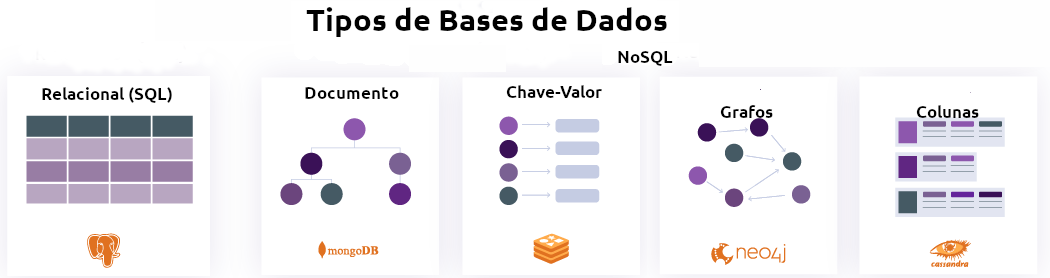
\includegraphics[width=0.8\textwidth]{../sty/NoSQL}
	\caption{Tipos de Bancos de Dados}
\end{figure}
